\documentclass[a4paper, 11pt]{article}
\usepackage{comment}
\usepackage{lipsum}
\usepackage{fullpage}
\usepackage[utf8]{inputenc}
\usepackage[T1]{fontenc}
\usepackage{libertine}
\usepackage{libertinust1math}
\usepackage{graphicx}
\usepackage{svg}
\graphicspath{ {images/} }


\begin{document}

\noindent
\large\textbf{Algorithmen und Datenstrukturen} \hfill \textbf{Christoph Stach (555912)} \\
\normalsize Aufgabe 3: Stack \hfill Tom Buhrtz \\

\section*{AufgabenBlatt 3 - 2}

\subsection*{Adjazenzmatrix}
\begin{tabular}{ |c|c|c|c|c|c|c| }
\hline
  & A & B & C & D & E & F \\
\hline
A & 0 & 0 & 0 & 0 & 0 & 0 \\
\hline
B & 0 & 0 & 0 & 0 & 0 & 0 \\
\hline
C & 0 & 0 & 0 & 0 & 0 & 0 \\
\hline
D & 0 & 0 & 0 & 0 & 0 & 0 \\
\hline
E & 0 & 0 & 0 & 0 & 0 & 0 \\
\hline
F & 0 & 0 & 0 & 0 & 0 & 0 \\
\hline
\end{tabular}

\subsection*{Adjazenzliste}


\subsection*{Mathematische Darstellung}
\( G = \{ V , X \} \) \\
\( V = \{ A , B , C , D , E , F \} \)  \\
\( \vec X = \{ (A,B) , (A,C) , (A,D) , (A,E) , (A,F) , (B,A) , (C,A) , (D,A) , (E,A) , (F,A) \} \)

\pagebreak

\section*{AufgabenBlatt 3 - 3}



%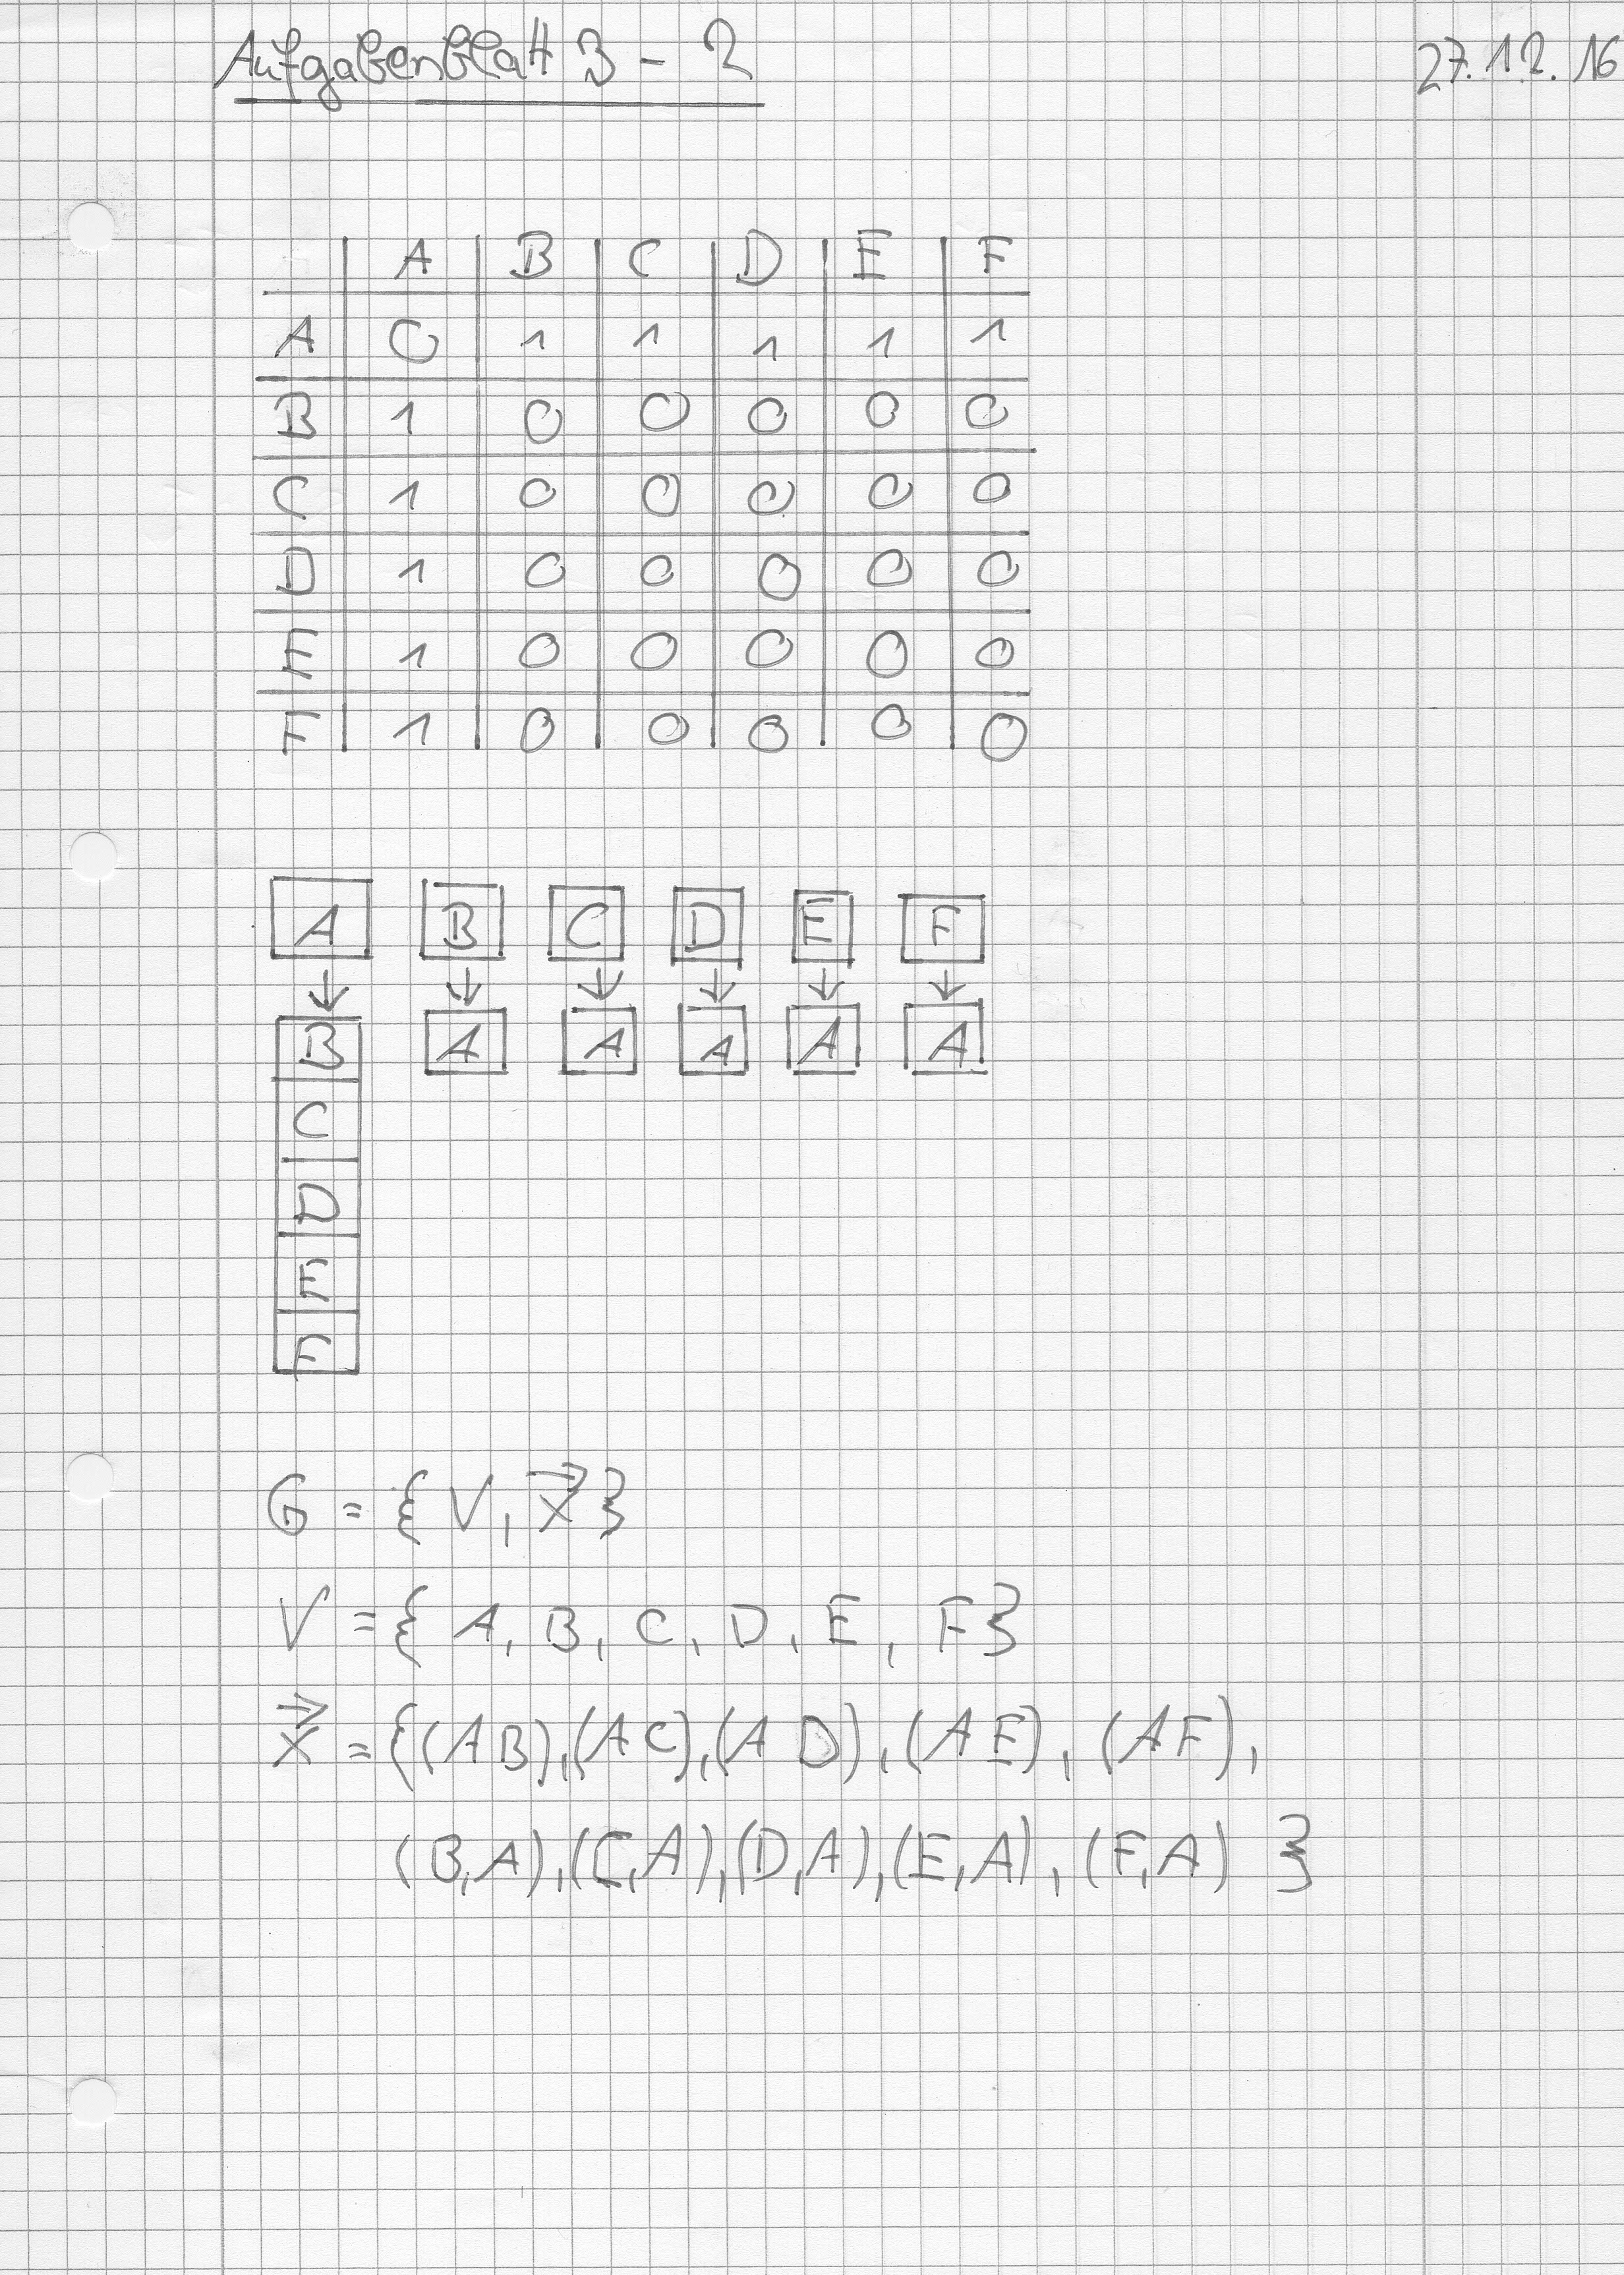
\includegraphics[width=15cm]{img-1}
%\pagebreak

%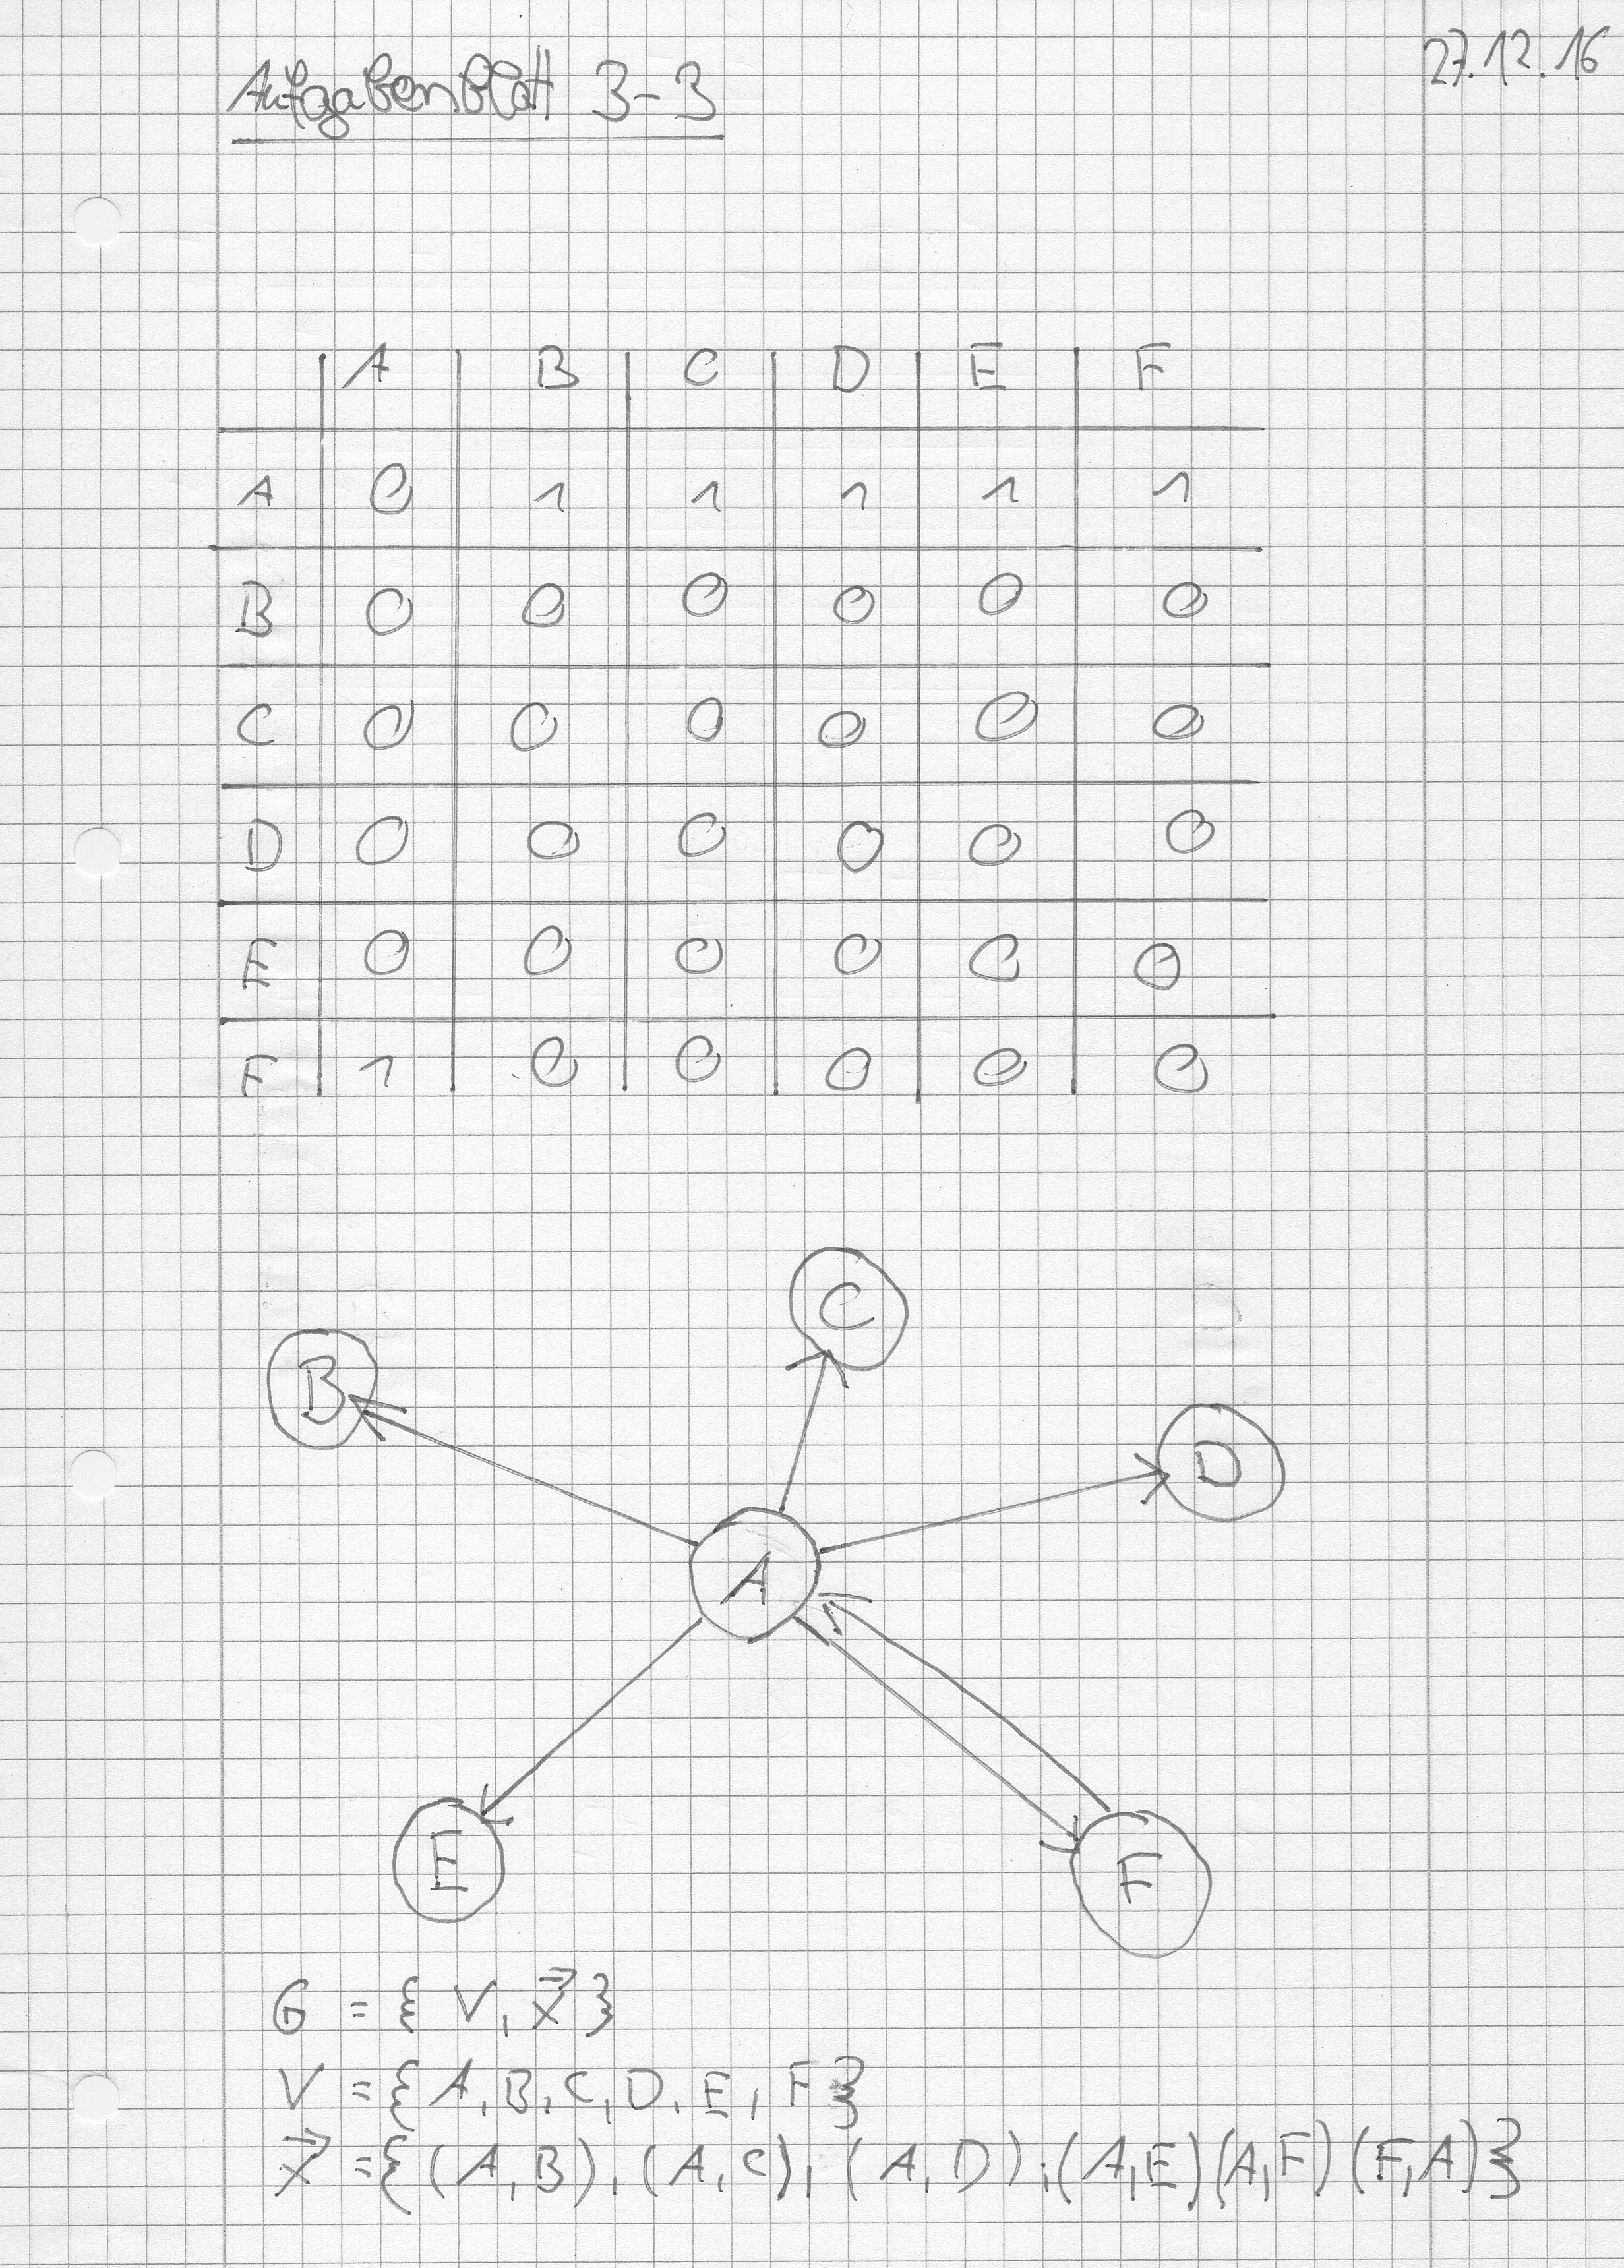
\includegraphics[width=15cm]{img-2}
%\pagebreak

%\includegraphics[width=15cm]{img-3}
%\pagebreak


\end{document}
